\part{Capítulo diez}

%----------------------------------------------------------------------------------------
%	CHAPTER 10
%----------------------------------------------------------------------------------------

\graphicspath{ {10_Capitulo/img/ejemplos/},{10_Capitulo/img/explicacion/}, {W_Varios/2_Portada_capitulos/} }


\chapterimage{ima2} % Chapter heading image

\chapter{Costo anual uniforme equivalente}

\section{Mapa Mental }
\begin{figure}[h]
	\centering
	\includegraphics[height=4.5cm]{Mapa Mental 10.1.pdf}\\
	\caption{Mapa mental CAUE}
\end{figure}

\section{Introducción}


El Costo Anual Uniforme Equivalente (CAUE), se basa en llevar todos los ingresos y egresos a una serie uniforme equivalente de pagos, de esta manera, los costos durante un año de una opción A se comparan con los costos durante un año de otra opción B.
Normalmente, el periodo de comparación es un año, no obstante, puede darse el caso de utilizar un periodo diferente, como es el caso del Costo Mensual Uniforme Equivalente (CMUE).
\\\\
La ventaja principal de este índice, es que no exige la toma de tiempos iguales como en el caso del valor presente neto (VPN), sino que únicamente se comparan los costos que en forma equivalente se hayan causado durante un año. También puede ser utilizado en aquellos casos en los que el uso del valor presente neto (VPN) se torna dispendioso, como el cálculo del mínimo común múltiplo de las vidas útiles de diferentes opciones para un ejercicio.


\newpage
\section{Fórmulas}

\begin{center}
	\begin{LARGE}
		\textbf{\[CAUE = VPN\left[ \frac{i(1+i)^n}{(1+i)^n-1}\right]\]}
	\end{LARGE}
\end{center}

Donde \textit{i} corresponde a la tasa de interés y \textit{n} a los periodos a evaluar.
\\\\
Es importante recordar que tiene aplicaciones en gestión y planeación de proyectos, si el resultado es positivo quiere decir que los ingresos son superiores a los egresos por tal motivo el proyecto puede llevarse a cabo, si su resultado es negativo quiere decir que los ingresos son inferiores que los egresos por consiguiente el proyecto no debe llevarse a cabo.

\subsection{Método del valor presente de salvamento}
El método del valor presente de salvamento es el segundo de los métodos para convertir a Costo Anual Uniforme Equivalente (CAUE) los costos de inversión que tengan valor de salvamento. El valor presente de salvamento se resta del costo de inversión inicial y la diferencia resultante se analiza para la vida del activo. La ecuación general es:
\begin{center}
	\begin{LARGE}
		\textbf{\[CAUE = P-VS+\left( \frac{P}{F}, i\%, n\right) \left( \frac{A}{P}, i\%, n\right) \]}
	\end{LARGE}
\end{center}

\subsection{Método de la recuperación de capital más intereses}
El procedimiento final que presentaremos aquí para el cálculo del Costo Anual Uniforme Equivalente (CAUE) de un activo que posea valor de salvamento, es el método de la recuperación de capital más intereses. La ecuación general para este método es:
\begin{center}
	\begin{LARGE}
		\textbf{\[CAUE = (P - VS) (AlP, i\%, n) + VS(i)\]}
	\end{LARGE}
\end{center}

\section{Ejemplos}

\textbf{Ejemplo 1}\\
Para realizar un proyecto se necesita realizar una inversión inicial de 80.000 COP y otra inversión de
45.000 COP al final del primer mes, en los meses 2 y 3 los ingresos son equivalentes a los egresos;
pero a partir del mes 4, se producen ingresos así: Mes cuatro 30.000 COP, mes cinco 50.000 COP, mes
seis 60.000 COP. Determinar si el proyecto lo pueden realizar los inversionistas A o B mencionados
anteriormente.\\


%%%%%%%%%%%%%%%%%%% EJERCICIO 1 %%%%%%

%\newpage %USAR SOLO SI EL SOLUCION QUEDA SOLO Y ES NECESARIO BAJARLO A LA SIGUIENTE PAGINA
\textbf{Solución.}\\
%La tabla ira centrada
\begin{center}
	\renewcommand{\arraystretch}{1.5}% Margenes de las celdas
	%Creacion de la cuadricula de 3 columnas \end{flushleft}
	\begin{longtable}[H]{|C{0.3\linewidth}|C{0.3\linewidth}|C{0.3\linewidth}|}
		%Creamos una linea horizontal
		\hline
         %%%%% INICIO FLUJO DE CAJA
		\rowcolor[HTML]{FFB183}
		\multicolumn{3}{|c|}{\cellcolor[HTML]{FFB183}\textbf{1. Asignación periodo focal}}   \\ \hline
		\multicolumn{3}{|c|} {$pf = 0 pmv$} \\ \hline
		%%%%%%%%%% FIN TITULO
		%%%%%%%%%% INICIO TITULO
		%Lo que se hace aqui es mezclar las 3 columnas en una sola
		\multicolumn{3}{|c|}{\cellcolor[HTML]{FFB183}\textbf{2. Declaración de variables}}   \\ \hline
		%%%%%%%%%% FIN TITULO
		%%%%%%%%%% INICIO DE MATEMATICAS
		%Cada & hace referencia al paso de la siguiente columna
		$n_{0} = 0 pmv$   & $n_{1} = 1 pmv$ & $n_{2} =  4 pmv$\\
		$n_{3} = 5 pmv$ & $n_{4} = 6 pmv$ & \\ \hline
		\multicolumn{3}{|c|}{$i_{a} = TIO_{a} = 3\% \equiv 0.03 pmv$} \\
		\multicolumn{3}{|c|}{$i_{b} = TIO_{b} = 2\% \equiv 0.02 pmv$} \\ \hline
		%%%%%%%%%% FIN DE MATEMATICAS
		%%%%% FIN DECLARACION DE VARIABLES


		%%%%% INICIO FLUJO DE CAJA
		\rowcolor[HTML]{FFB183}
		\multicolumn{3}{|c|}{\cellcolor[HTML]{FFB183}\textbf{3. Diagrama de flujo de caja}} \\ \hline
		%Mezclamos 3 columnas y ponermos el dibujo
		%%%%%%%%%%%%% INSERCION DE LA IMAGEN
		%Deberan descargar las imagenes respectivas del drive y pegarlas en la carpeta
		%n_capitulo/img/ejemplos/1/capitulo1ejemplo1.pdf  (el /1/ es el numero del ejemplo)
		\multicolumn{3}{|c|}{ 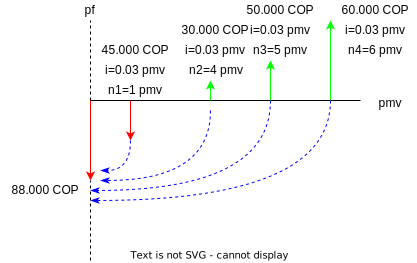
\includegraphics[trim=-5 -5 -5 -5 , scale=1.0,width=300px, height=250px]{9_Capitulo/ejemplos/1/Capitulo9Ejercicio1.pdf} }   \\ \hline
		%%%%%%%%%%%%% FIN INSERCION DE IMAGEN
		%%%%%FIN FLUJO DE CAJA



		%%%%% INICIO DECLARACION FORMULAS
		%%%%%%%%%%% INICIO TITULO
		\rowcolor[HTML]{FFB183}
		\multicolumn{3}{|c|}{\cellcolor[HTML]{FFB183}\textbf{4. Declaración de fórmulas}}    \\ \hline
		%%%%%%%%%%% FIN TITULO
		%%%%%%%%%%% INICIO MATEMATICAS
		\multicolumn{3}{|c|}{$\sum F_{n}(1+i)^{-n} $\hspace{0.3cm} \textit{Valor presente neto}} \\ \hline
		%%%%%%%%%% FIN MATEMATICAS
		%%%%%% INICIO DESARROLLO MATEMATICO
		\rowcolor[HTML]{FFB183}
		%%%%%%%%%%INICIO TITULO
		\multicolumn{3}{|c|}{\cellcolor[HTML]{FFB183}\textbf{5. Desarrollo matemático}}       \\ \hline
		%%%%%%%%%% FIN TITULO
		%%%%%%%%%% INICIO MATEMATICAS
		\multicolumn{3}{|c|}{$VPN_{a} = -80000 - 45000(1+0.03)^{-1} + 30000(1+0.03)^{-4} + 50000(1+0.03)^{-5} + 60000(1+0.03)^{-6}$} \\
		\multicolumn{3}{|c|}{$VPN_{a} = -3655$} \\
		\multicolumn{3}{|c|}{$VPN_{b} = -80000 - 45000(1+0.02)^{-1} + 30000(1+0.02)^{-4} + 50000(1+0.02)^{-5} + 60000(1+0.02)^{-6}$} \\
		\multicolumn{3}{|c|}{$VPN_{b} = 216254$} \\ \hline

		%%%%%%%%%% FIN MATEMATICAS
		%%%%%% FIN DESARROLLO MATEMATICO
		%%%%%% INICIO RESPUESTA
		\rowcolor[HTML]{FFB183}
		%%%%%%%%%%INICIO TITULO
		\multicolumn{3}{|c|}{\cellcolor[HTML]{FFB183}\textbf{6. Respuesta}}   \\ \hline
		%%%%%%%%%% FIN TITULO
		%%%%%%%%%% INICIO RESPUESTA MATEMATICA
		\multicolumn{3}{|c|}{Para B el $VPN > 0$, significa que puede realizar el proyecto en pesos de hoy,} \\ 
		\multicolumn{3}{|c|}{además de ganarse el 2\%, obtiene una ganancia de 2.162,54 COP.}  \\ \hline
		%%%%%%%%%% FIN MATEMATICAS
		%%%%%% FIN RESPUESTA
	\end{longtable}
	%Se crean dos lineas en blanco para que no quede el siguiente texto tan pegado
	%\newline \newline %USARLO SI CREES QUE ES NECESARIO
\end{center}
%%%%%%%%%%%%%%%%%%%%%%%%%%FIN EJERCICIO 1 %%%%%%%%%%%%%%%%%%%%%%%%%%%


\textbf{Ejemplo 2}\\
Se invierten 200{.}000 COP en un depósito a término fijo de 6 meses en un banco que paga el 28\% namv. Determinar el monto de la entrega al vencimiento.\\

%%%%%%%%%%%%%%%%%%% EJERCICIO 1 %%%%%%

%\newpage %USAR SOLO SI EL SOLUCIÓN QUEDA SOLO Y ES NECESARIO BAJARLO A LA SIGUIENTE PAGINA
\textbf{Solución.}
%La tabla ira centrada
\begin{center}
  \renewcommand{\arraystretch}{1.5}% Margenes de las celdas
  %Creación de la cuadricula de 3 columnas \end{flushleft}
  \begin{longtable}[H]{|C{0.3\linewidth}|C{0.3\linewidth}|C{0.3\linewidth}|}
    %Creamos una linea horizontal
    \hline
    %Definimos el color de la primera fila
    \rowcolor[HTML]{FFB183}
    %%%%% INICIO ASIGNACIÓN FECHA FOCAL %%%%%%%
    %%%%%%%%%% INICIO TITULO
    %Lo que se hace aquí es mezclar las 3 columnas en una sola
    \multicolumn{3}{|c|}{\cellcolor[HTML]{FFB183}\textbf{1. Asignación período focal}}                                  \\ \hline
    %%%%%%%%%% FIN TITULO
    %%%%% INICIO DECLARACIÓN DE VARIABLES %%%%%%%
    \multicolumn{3}{|c|}{$pf = 6pmv$}                                                                                   \\ \hline
    %%%%%%%%%% INICIO TITULO
    %Lo que se hace aquí es mezclar las 3 columnas en una sola
    \multicolumn{3}{|c|}{\cellcolor[HTML]{FFB183}\textbf{2. Declaración de variables}}                                  \\ \hline
    %%%%%%%%%% FIN TITULO
    %%%%%%%%%% INICIO DE MATEMÁTICAS
    %Cada & hace referencia al paso de la siguiente columna
    $P =  200{.}000$ COP & $n = 6\textit{pmv} $ & $i= ?\% pmv$                                                           \\
    $j=28\%namv$         & $m=12pmv$            & $F = ? COP$                                                           
    \\\hline

    %%%%%%%%%% FIN DE MATEMÁTICAS
    %%%%% FIN DECLARACIÓN DE VARIABLES


    %%%%% INICIO FLUJO DE CAJA
    \rowcolor[HTML]{FFB183}
    \multicolumn{3}{|c|}{\cellcolor[HTML]{FFB183}\textbf{3. Diagrama de flujo de caja}}                                 \\ \hline
    %Mezclamos 3 columnas y pondremos el dibujo
    %%%%%%%%%%%%% INSERCIÓN DE LA IMAGEN
    %Deberán descargar las imágenes respectivas del drive y pegarlas en la carpeta
    %n_capitulo/img/ejemplos/1/capitulo1ejemplo1.pdf  (el /1/ es el numero del ejemplo)
    \multicolumn{3}{|c|}{ 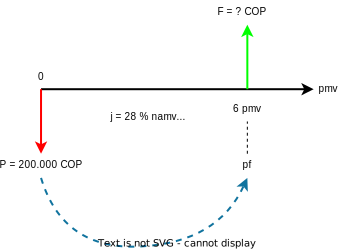
\includegraphics[trim=-5 -5 -5 -5 , scale=1]{2_Capitulo/ejemplos/2/Capitulo2Ejercicio2_v2.pdf} } \\ \hline
    %%%%%%%%%%%%% FIN INSERCIÓN DE IMAGEN
    %%%%%FIN FLUJO DE CAJA



    %%%%% INICIO DECLARACIÓN FORMULAS
    %%%%%%%%%%% INICIO TITULO
    \rowcolor[HTML]{FFB183}
    \multicolumn{3}{|c|}{\cellcolor[HTML]{FFB183}\textbf{4. Declaración de fórmulas}}                                   \\ \hline
    %%%%%%%%%%% FIN TITULO
    %%%%%%%%%%% INICIO MATEMÁTICAS
    \multicolumn{3}{|c|}{$F = P(1+i)^n \hspace{0.3cm} \textit{Valor futuro}$}                                           \\
    \multicolumn{3}{|c|}{$j=i\cdot m\hspace{0.3cm}\textit{Tasa periódica anualizada}$}
    \\ \hline
    %%%%%%%%%% FIN MATEMÁTICAS
    %%%%%% INICIO DESARROLLO MATEMÁTICO
    \rowcolor[HTML]{FFB183}
    %%%%%%%%%%INICIO TITULO
    \multicolumn{3}{|c|}{\cellcolor[HTML]{FFB183}\textbf{5. Desarrollo matemático}}                                     \\ \hline
    %%%%%%%%%% FIN TITULO
    %%%%%%%%%% INICIO MATEMÁTICAS
    \multicolumn{3}{|c|}{$0{.}28=i\cdot 12$}                                                                            \\
    \multicolumn{3}{|c|}{$i= \frac{0{.}28}{12} = 0{.}02333... \equiv 2{.}333\%pmv$}                                     \\
    \multicolumn{3}{|c|}{$0{.}28=i\cdot 12$}                                                                            \\
    \multicolumn{3}{|c|}{$F = 200{.}000 COP(1+0,2333)^6$}                                                       \\
    \multicolumn{3}{|c|}{$F = 229{.}685.04 COP$}
    \\ \hline


    %%%%%%%%%% FIN MATEMÁTICAS
    %%%%%% FIN DESARROLLO MATEMÁTICO
    %%%%%% INICIO RESPUESTA
    \rowcolor[HTML]{FFB183}
    %%%%%%%%%%INICIO TITULO
    \multicolumn{3}{|c|}{\cellcolor[HTML]{FFB183}\textbf{6. Respuesta}}                                                 \\ \hline
    %%%%%%%%%% FIN TITULO
    %%%%%%%%%% INICIO RESPUESTA MATEMÁTICA
    \multicolumn{3}{|c|}{$F = 229{.}685.04 COP$
    }                                                                                                                   \\ \hline
    %%%%%%%%%% FIN MATEMÁTICAS
    %%%%%% FIN RESPUESTA
  \end{longtable}
  %Se crean dos lineas en blanco para que no quede el siguiente texto tan pegado
  %\newline \newline %USARLO SI CREES QUE ES NECESARIO
\end{center}
%%%%%%%%%%%%%%%%%%%%%%%%%%FIN EJERCICIO 1 %%%%%%%%%%%%%%%%%%%%%%%%%%%


\textbf{Ejemplo 3}\\
Una fabrica produce actualmente en forma manual 1.000 unidades de un determinado artículo, para ello utiliza artesanos a los cuales les paga 8.400.000 COP al año y, es costumbre que cada año se les aumente el sueldo en aproximadamente un 20\%. El precio de venta de cada artículo es de 9.000 COP y se estima que este precio podrá ser aumentado todos los años en un 21\%. Ahora se ha presentado la oportunidad de adquirir una máquina a un costo de 10 millones COP con una vida útil de 5 años; un valor de salvamento de 2 millones COP la cual requiere de 2 técnicos para su operación, el sueldo anual de cada uno de los técnicos puede ser de 600.000 COP con aumentos anuales de sueldo del 20\% ¿Cuál de las dos alternativas es mejor suponiendo que la tasa del inversionista es del 30\%?\\


%%%%%%%%%%%%%%%%%%% EJERCICIO 3 %%%%%%

%\newpage %USAR SOLO SI EL SOLUCION QUEDA SOLO Y ES NECESARIO BAJARLO A LA SIGUIENTE PAGINA
\textbf{Solución.}\\
%La tabla ira centrada
\begin{center}
	\renewcommand{\arraystretch}{1.5}% Margenes de las celdas
	%Creacion de la cuadricula de 3 columnas \end{flushleft}
	\begin{longtable}[H]{|C{0.3\linewidth}|C{0.3\linewidth}|C{0.3\linewidth}|}
		%Creamos una linea horizontal
		\hline
        %%%%% INICIO FLUJO DE CAJA
		\rowcolor[HTML]{FFB183}
		\multicolumn{3}{|c|}{\cellcolor[HTML]{FFB183}\textbf{1. Asignación periodo focal}}   \\ \hline
		\multicolumn{3}{|c|} {$pf = 0 pav$} \\ \hline
		%%%%%%%%%% FIN TITULO
		%%%%%%%%%% INICIO TITULO
		%Lo que se hace aqui es mezclar las 3 columnas en una sola
		\multicolumn{3}{|c|}{\cellcolor[HTML]{FFB183}\textbf{2. Declaración de variables}}   \\ \hline
		%%%%%%%%%% FIN TITULO
		%%%%%%%%%% INICIO DE MATEMATICAS
		%Cada & hace referencia al paso de la siguiente columna
		$R_{1} = 9.000.000 $ COP   & $R_{2} = 8.400.000$ COP  & $i=0.3pav$\\ 
		$g_{1} =  0.21 pav $ & $g_{2}=  0.2 pav $ & $n=5pav$ \\ \hline
		%%%%%%%%%% FIN DE MATEMATICAS
		%%%%% FIN DECLARACION DE VARIABLES

  		%%%%% INICIO DECLARACION FORMULAS
  
		%%%%%%%%%%% INICIO TITULO
		\rowcolor[HTML]{FFB183}
		\multicolumn{3}{|c|}{\cellcolor[HTML]{FFB183}\textbf{3. Diagrama de flujo de caja}} \\ \hline
		%Mezclamos 3 columnas y ponermos el dibujo
		%%%%%%%%%%%%% INSERCION DE LA IMAGEN
		%Deberan descargar las imagenes respectivas del drive y pegarlas en la carpeta
		%n_capitulo/img/ejemplos/1/capitulo1ejemplo1.pdf  (el /1/ es el numero del ejemplo)
		\multicolumn{3}{|c|}{ \includegraphics[trim=-5 -5 -5 -5 , scale=1, width=300px, height=250px]{9_Capitulo/ejemplos/3/Capitulo9Ejercicio3.pdf} }   \\ \hline
		%%%%%%%%%%%%% FIN INSERCION DE IMAGEN
		%%%%%FIN FLUJO DE CAJA



		%%%%% INICIO DECLARACION FORMULAS
		%%%%%%%%%%% INICIO TITULO
		\rowcolor[HTML]{FFB183}
		\multicolumn{3}{|c|}{\cellcolor[HTML]{FFB183}\textbf{4. Declaración de fórmulas}}    \\ \hline
		%%%%%%%%%%% FIN TITULO
		%%%%%%%%%%% INICIO MATEMATICAS
		\multicolumn{3}{|c|}{$\sum F_{n}(1+i)^{-n} $\hspace{0.3cm} \textit{Valor presente neto}} \\ \hline
		%%%%%%%%%% FIN MATEMATICAS
		%%%%%% INICIO DESARROLLO MATEMATICO
		\rowcolor[HTML]{FFB183}
		%%%%%%%%%%INICIO TITULO
		\multicolumn{3}{|c|}{\cellcolor[HTML]{FFB183}\textbf{5. Desarrollo matemático}}       \\ \hline
		%%%%%%%%%% FIN TITULO
		%%%%%%%%%% INICIO MATEMATICAS
		\multicolumn{3}{|c|}{$VPN_{A} = \frac{9[(1+0.21)^{5}(1+0.3)^{-5} -1]}{0.21-0.3} - \frac{8.4[(1+0.2)^{5}(1+0.3^{-5} -1)]}{0.2-0.3}$} \\
		\multicolumn{3}{|c|}{$VPN_{A} = 2.437.836 $ COP} \\
		\multicolumn{3}{|c|}{$VPN_{B} = \frac{9[(1+0.21)^{5}(1+0.3)^{-5} -1]}{0.21-0.3} + 2(1.3)^{-5} - \frac{1.2[(1+0.2)^{5}(1+0.3^{-5} -1)]}{0.2-0.3}$} \\
		\multicolumn{3}{|c|}{$VPN_{B} = 16.723.756 $ COP} \\ \hline

		%%%%%%%%%% FIN MATEMATICAS
		%%%%%% FIN DESARROLLO MATEMATICO
		%%%%%% INICIO RESPUESTA
		\rowcolor[HTML]{FFB183}
		%%%%%%%%%%INICIO TITULO
		\multicolumn{3}{|c|}{\cellcolor[HTML]{FFB183}\textbf{6. Respuesta}}   \\ \hline
		%%%%%%%%%% FIN TITULO
		%%%%%%%%%% INICIO RESPUESTA MATEMATICA
		\multicolumn{3}{|c|}{La decisión correcta es comprar la máquina.}  \\ \hline
		%%%%%%%%%% FIN MATEMATICAS
		%%%%%% FIN RESPUESTA
	\end{longtable}
	%Se crean dos lineas en blanco para que no quede el siguiente texto tan pegado
	%\newline \newline %USARLO SI CREES QUE ES NECESARIO
\end{center}
%%%%%%%%%%%%%%%%%%%%%%%%%%FIN EJERCICIO 3 %%%%%%%%%%%%%%%%%%%%%%%%%%%

